% (c) 2020 Stefan Antonowicz
% Based off of tex found at https://github.com/ludus-leonis/nipajin
% This file is released under Creative Commons Attribution-NonCommercial-ShareAlike 4.0 International License.
% Please do not apply other licenses one-way.

\renewcommand{\yggAdvancement}{%
  \mychapter{Advancement}{advancement}
  \mysectionheader{advancement/AdvancementHeader}
  \newpage
}

\renewcommand{\yggAdvancementText}{%

\mysection{Glory}{advancement-glory}

The longer lived your Adventurer, the more they increase in skill and power, represented by \mybold{Glory}. You earn Glory during \mylink{Downtime}{downtime}; when you gain enough Glory, you go up in Level, which grants you more \mylink{Grit}{adventurer-flesh-grit} and additional powers. The higher you go in \LVL, the more Glory you'll need to acquire. 

During the \mylink{Training Step}{downtime-training} of \mylink{Downtime}{downtime}, you may convert your coin into Glory. The exchange rate depends on your level. You can spend enough coin to raise yourself to the next level, but not any further.

\callout {
    \mybullet {
        \item  At Levels 1 and 2, you get 1 Glory for each \mybold{Iron piece} you convert. A Silver piece is worth 10 Glory, and a Gold piece is worth 100 Glory.
        \item  At Levels 3, 4, and 5, you get 1 Glory for each \mybold{Silver piece} you convert. A Gold piece is worth 10 Glory. Iron pieces can't be converted.
        \item  At Levels 6+, you get 1 Glory for each \mybold{Gold piece} you convert. Iron and Silver pieces can't be converted.
    }
}

Converting coin to Glory in this way assumes you've been bribing sorcerers and librarians, buying books, paying someone to spar with, etc. You’ll note that it gets harder and harder to gain Glory with money as you go up in level. This is by design - legendary heroes aren’t getting Glory taking money from orc babies, but by doing epic shit. In time, the jewels cease to sparkle...

\mysubsection{Adventure}{glory-adventure}


The meta section of \mylink{the Game}{time-adventure} defines an Adventure as one or more Sessions. When your \mylink{Band}{roles-band} writes the last line of a chapter of their exploits, they complete an Adventure  (for example: Thundarr breaks the werewolf curse; Conan escapes the Demons of the Summit; Fafhrd and the Grey Mouser return to Lankhmar with Ohmphal's fingertips, etc.).  During the \mylink{The Arbiter's Step}{downtime-arbiter} of \mylink{Downtime}{downtime}, after you spend your coin, the Arbiter has a chance to award you additional Glory for the adventures you just survived.  This Glory might be for your entire Band, or it might be for an individual member; it might be enough to put you at the next level, or it might be enough to leave you shy by 1.  The Arbiter gets final say no matter what.  See the Arbiter's Step section under Downtime for more info.


\mysection{Levels}{advancement-levels}

Levels and Ranks are measures of how powerful you have become.  Every Adventurer starts as a Level 1 Greenhorn. The more Glory you win, the higher your Level and Rank:

  \mytable{X X X X}{
    \thead{Level} & \thead{Rank} & \thead{Min Glory} & \thead{Coin Type} \\
  }{
    1 & Greenhorn &  0 & Iron \\
    2 & Daredevil &  1,000 & Iron \\
    3 & Daredevil &  3,000 & Silver \\
    4 & Hero &  6,000 & Silver \\
    5 & Hero &  11,000 & Silver \\
    6 & Hero &  19,000 & Gold \\
    7 & Legend  & 32,000 & Gold \\
    8 & Legend  & 53,000 & Gold \\
    9 & Demigod & 87,000 & - \\    
}

Whenever you gain enough Glory to advance to the next level, your Grit goes up. Immediately roll your \INSANITY, \DEATH, and \INJURY dice (your \mylink{Kismet}{adventurer-kismet}) and add their total to your \MAX \mylink{Grit}{adventurer-flesh-grit}. Then, find your Trope or Species below and \mybold{choose 3} of the of the Daredevil, Heroic, and/or Legendary Virtues beneath.  

\mybold{You can choose Daredevil Virtues at any level, Heroic Virtues at level 4+, and Legendary Virtues at level 7+}.


\newpage

\myimage{advancement/SeatedWizard}

\cbreak

\mysubsection{Arbiter's Awards}{advancement-arbiters-awards}

At the Arbiter's complete discretion, you may be awarded extra perks based on how "heroic" your last level was. These perks can vary as the Arbiter sees fit, but should always be beneficial. Some examples from our campaigns:

    \mybullet {
        \item +4 Grit awarded to a Knave who risked being burned alive to have a "Michael Bay" moment as they walked away from an explosion;
        \item +1 Flesh awarded to a Philosopher who failed their Mishap roll three times in a single Session, and became part pig, part goat, and part rooster;
        \item +1 Save vs. Doom awarded to a Sellsword who made 6 consecutive Saves vs. Doom battling a horde of paralytic undead;
        \item etc.
    }


% single page for this section
\end{multicols*}
\newpage
\mysection{Tropes}{advancement-tropes}
  %%%%%%%%%%%%%%%%%%%%%%%%%%%%%%%%%%%%%%%%%%%%%%%%%%%%%%%%%%%%%%%%%%%%%%
  %%%%  KNAVE %%%%%%%%%%%%%%%%%%%%%%%%%%%%%%%%%%%%%%%%%%%%%%%%%%%%%%%
  %%%%%%%%%%%%%%%%%%%%%%%%%%%%%%%%%%%%%%%%%%%%%%%%%%%%%%%%%%%%%%%%%%%%%%


\mysubsection{Knave Virtues}{advancement-knave-virtues}

\myemph{Unless otherwise specified, you can take each Virtue only once.}


  \mytable{Y Y Y} {
    \thead{Daredevil (Level 2+)} & \thead{Heroic (Level 4+)} & \thead{Legendary (Level 7+)} \\
  } {
    Beginner's Luck & Kismet II & Astonishing Luck \\
    Charms & Left Hand Path (Sharper)\Asterisk  & Guildmaster \\
    Deadeye & Personality II & Kismet III \\
    Kismet I & Precepts of Blight & Left-Hand Path (Master)\Asterisk \\
    Left-Hand Path (Apprentice)\Asterisk & Precepts of Blood & Personality III \\
    Left-Hand Path (Footpad)\Asterisk & Precepts of Celerity & The Plan \\
    Medicine & Precepts of Wizardry & Saves III \\
    Mummy's Curse & Saves II & Surprise Motherfucker! \\
    Personality I & Uncanny Luck & - \\
    Sacraments & Unlabeled Package & - \\
    Saves I & - & - \\
    Slippery &  - & - \\
}

\callout {
    \Asterisk This Virtue can be taken once per \LVL. See details in description.
}


\begin{multicols*}{2}

\myhighlight{Astonishing Luck}{adv-knave-virtue-astonishing-luck}

Advance your \mypg{Lucky Die}{knave-lucky-die} \DCUP.

\myhighlight{Beginner's Luck}{adv-knave-virtue-beginners-luck}

Advance your \mypg{Lucky Die}{knave-lucky-die} \DCUP.

\myhighlight{Charms}{adv-knave-virtue-charms}

You can perform the \mypg{Vulgate of Charms}{vulgate-charms} at will.

\myhighlight{Deadeye}{adv-knave-virtue-deadeye}

Identical to the Virtue of the same name under the \mypg{Knave Trope}{trope-knave}. 

\cbreak

\myhighlight{Guildmaster}{adv-knave-virtue-guildmaster} 

You become the grandmaster of a new Thieves Guild. Choose a Medium or Large Settlement where your guild is located. When you take Downtime in this Settlement, you will be given information, food, and lodging for free. When figuring out how much coin you must pay for resting, treat the length of your stay as if it were one step less expensive i.e. treat Months as if you were staying for Weeks; Weeks for Days; and Days cost you nothing (staying for Years still costs the same, however). The Arbiter must share a rumor with you about your current or next adventure - the clue might be obscure, but it must be true.

If you desire, 2 footpads will join you on your next adventure.  They are \mypg{Mercenaries}{gear-mercenaries} in all ways like \mybold{Mechanics}, except they have a starting Loyalty of 9, wear Leather Armor, and have no trouble working together. In Combat, you have to specify what each footpad is doing at the top of each Moment i.e. "1 is giving me +1 damage and I'm keeping one back to take damage in case things go south." Outside of Combat, each footpad can provide you with a +1 on any Whisper tries. If a footpad dies or leaves your service, you can replace them with another during the Production Step of Downtime. Note that if your footpads often meet with an untimely end, starve to death, leave your service, etc. you may begin to develop a ... reputation ... at the Arbiter's discretion.

You are encouraged to work out additional details with the Arbiter, and let the Arbiter know the name of your guild.


\myhighlight{Kismet I-III}{adv-knave-virtue-kismet}

Advance \mybold{all} aspects of your \mybold{Kismet} - \DEATH, \INJURY, and \INSANITY - to the next named level. 

\myhighlight{Left-Hand Path (Apprentice)}{adv-knave-virtue-left-hand-path-apprentice}

Advance any two Whispers from Untrained to Apprentice (d4) rank. You can take this Virtue more than once.

\myhighlight{Left-Hand Path (Footpad)}{adv-knave-virtue-left-hand-path-footpad}

Advance any two Whispers from Apprentice to Footpad (d6) rank. You can take this Virtue more than once.

\myhighlight{Left-Hand Path (Sharper)}{adv-knave-virtue-left-hand-path-sharper}

Advance any two Whispers from Footpad to Sharper (d8) rank. You can take this Virtue more than once.

\myhighlight{Left-Hand Path (Master)}{adv-knave-virtue-left-hand-path-master}

Advance any two Whispers from Sharper to Master (d10) rank. You can take this Virtue more than once.

\myhighlight{Medicine}{adv-knave-virtue-medicine}

You can perform the \mypg{Vulgate of Medicine}{vulgate-medicine} during the Shopping Step of Downtime. 

\myhighlight{Mummy's Curse}{adv-knave-virtue-mummys-curse}

Identical to the Virtue of the same name under the Knave Trope

\myimage{advancement/DeerSkulls}

\myhighlight{Personality I-III}{adv-knave-virtue-personality}

Advance two \mybold{different} aspects of your \mybold{Personality} \DCUP.

\myhighlight{The Plan}{adv-knave-virtue-the-plan} 

Once per Session, you can declare that you’ve been planning for this very situation all along. Everyone in the group gets +4 to all \RO attempts for d6 real-world minutes.  You need to tell the Arbiter how you influenced prior actions to lead to this outcome. 

\myhighlight{Precepts of Blight}{adv-knave-virtue-blight} 

You have 2 Research Pips that you may use during the Production Step of Downtime to create an Acid or Toxin (only). See the section on \mypg{Research: Chymistry}{research-chymistry} for more info.

\myhighlight{Precepts of Blood}{adv-knave-virtue-blood} 

You may Murder someone using a Mace, Spear, Sword, or War Axe.

\myhighlight{Precepts of Celerity}{adv-knave-virtue-celerity} 

Your \MD when wearing Light Armor is d20.

\myhighlight{Precepts of Wizardry}{adv-knave-virtue-wizardry} 

When reading a Secret from a Fetish, the Fetishes' \UD only moves \DCDOWN on a 1 (instead of a 1 or 2).

\myhighlight{Sacraments}{adv-knave-virtue-sacraments}

You gain a single Grace die (d4) which allows you to perform the \mypg{Sacraments}{vulgate-sacraments}.

\myhighlight{Saves I-III}{adv-knave-virtue-saves}

Advance \mybold{all} Saves to the next named level (Defenseless to Preserved; Preserved to Protected; etc).

\cbreak

\myhighlight{Slippery}{adv-knave-virtue-slippery}

Once per Session, you can automatically escape from something that is restraining you and that you could plausibly escape from. This includes grapples, lynchings, and awkward social situations, but not sealed coffins.

\myhighlight{Surprise, Motherfucker!}{adv-knave-virtue-surprise-motherfucker} 

Once per Adventure, at any time, you may declare that you are walking off-screen. During any Session of the Adventure, you may reveal yourself to have been a minor NPC in the background of the scene "all along" as long as there are minor NPCs in the background of the scene. You can always walk back on stage at any time, even climbing in a window. This ability is limited by plausibility (Arbiter's discretion). 

\myhighlight{Uncanny Luck}{adv-knave-virtue-uncanny-luck} 

Advance your \mypg{Lucky Die}{knave-lucky-die} \DCUP.

\myhighlight{Unlabeled Package}{adv-knave-virtue-unlabeled-package} 

In a Medium or Large Settlement, you may spend any amount of money during the Shopping Step of Downtime to buy an Unlabeled Package. When the package is unwrapped, you declare what it contains, provided (a) it didn't cost more than you originally paid, (b) it's smaller than a 1m cube, (c) wouldn't be more than 1 Burden  (no storing 100,000\AU in an Unlabeled package, for example), (d) is mundane, and (e) would be available in the Settlement where you purchased it.


\end{multicols*}

\newpage
%%%%%%%%%%%%%%%%%%%%%%%%%%%%%%%%%%%%%%%%%%%%%%%%%%%%%%%%%%%%%%%%%%%%%%
%%%%  MYSTIC %%%%%%%%%%%%%%%%%%%%%%%%%%%%%%%%%%%%%%%%%%%%%%%%%%%%%%%
%%%%%%%%%%%%%%%%%%%%%%%%%%%%%%%%%%%%%%%%%%%%%%%%%%%%%%%%%%%%%%%%%%%%%%

\mysubsection{Mystic Virtues}{advancement-mystic-virtues}

\begin{center}
\myredbold{Unless otherwise specified, you can only take each Virtue once.}
\end{center}


  \mytable{Y Y Y} {
    \thead{Daredevil (Level 2+)} & \thead{Heroic (Level 4+)} & \thead{Legendary (Level 7+)} \\
  } {
    Charms  & Cloister & Charmed Circle \\
    Cunning Folk\Asterisk & Feyness & Fishers of Men \\
    Devotion\Asterisk & Kismet II  & Kismet III \\
    Kismet I & Liturgies of the Apostles &  Liturgies of the Saints  \\
    Liturgies of the Clerics  & Master of Puppets & Necromancer \\
     Liturgies of the Novitiates & Personality II & Norn's Shears \\
     Medicine & Saves II & Personality III \\
     Mombo\Asterisk   & Tongues of Fire & Saves III \\
    Personality I  & Uncanny & - \\
    Sacraments & Witch & - \\
     Saves I & - & - \\
     Wisdom & - & - \\
}

\callout {
    \Asterisk This Virtue can be taken once per \LVL. See details in description
}

\begin{multicols*}{2}




\myhighlight{Charmed Circle}{adv-mystic-charmed-circle}

When taking \mylink{Downtime}{downtime} in a Settlement that has a \mylink{Locus}{gear-services-loci}, your brothers and sister will offer you aid and succor. They will give you information, food, and lodging for free. When figuring out how much coin you must pay for resting, treat the length of your stay as if it were one step less expensive i.e. treat Months as if you were staying for Weeks; Weeks for Days; and Days cost you nothing (staying for Years still costs the same, however). At your behest, \mylink{Mundungu}{gear-services} will summon Hekaphage to eat curses either for free or for trade (Arbiter's discretion). The amount of time to create \mylink{Marvels}{cunning-marvels} is shortened to Days; \mylink{Occultism}{cunning-marvels} that takes Months takes only Weeks, and Weeks only takes Days. Finally, the Charmed Circle grants you 4 extra Cunning Pips to use as you wish.

\myhighlight{Charms}{adv-mystic-charms}

You can perform the \mylink{Charms}{vulgate-charms} Vulgate at will.

\cbreak

\myhighlight{Cloister}{adv-mystic-cloister}

Depending on the size of the Settlement you're in, you have a chance (Small: 25\%, Medium 75\%, Large 100\%) of finding other practitioners of your faith - a coven, cult, church, or what-have-you.  Your brethren will give you information, food, and lodging for free. When figuring out how much coin you must pay for resting, treat the length of your stay as if it were one step less expensive i.e. treat Months as if you were staying for Weeks; Weeks for Days; and Days cost you nothing (staying for Years still costs the same, however). The Arbiter must share a rumor with you about your current or next adventure - the clue might be obscure, but it must be true.

\myhighlight{Cunning Folk}{adv-mystic-cunning-folk}

Identical to the Virtue of the same name under the \mylink{Mystic Trope}{trope-mystic}. If you already know this Virtue, gain 1 Cunning Pip. You can choose this Virtue once per Level.

\myimage{advancement/Mystic4}

\myhighlight{Devotion}{adv-mystic-devotion}

Gain +1 \MAX Faith, and 1 Faith Die. You can choose this Virtue once per Level.


\myhighlight{Feyness}{adv-mystic-feyness}

You can detect magic, supernatural effects, and general weirdness. 30m range for minor enchantments, charms, and sorceries; 1km range for seriously worrying magical trouble. It might be a premonition, a vision, a cold shudder, a glowing aura, or just a sense that something is "wrong". You can see ghosts and spirits, and they will know and respect you (you never need to roll \INSANITY for seeing shades or horrors). You know if an item is magical by inspecting it for Minutes.

\myhighlight{Fishers of Men}{adv-mystic-fishers-of-men}

If you take \mylink{Downtime}{downtime} in a Settlement that has a \mylink{Shrine}{gear-services-shrines} dedicated to your Small God, a member of the faithful will seek you out during the \mylink{Production Step}{downtime-production}.  If you desire, you may give this adherent one of your Faith Die to make them into a \mybold{Disciple}. The Faith die is Spent, but now resides inside of the Disciple.  Whenever you take Downtime in this Settlement, you may call upon your Disciple(s) to assist you in your \mylink{Miracle working}{wonders-miracles}. You may use the Faith die of a Disciple as if it were your own; this Faith Die can only be used once during Downtime, but will not become Spent. Should you ever suffer a \mylink{Crisis of Faith}{cruces-faith-dice-recovery}, your Disciples will immediately leave your service (even if you are not in the Settlement where they reside). You can never have more than 12 Disciples (including Vassals and Crusaders), and your Disciples will not leave the Settlement where they were first converted. They will proselytize the faith of your Small God in your absence, for good or ill.

\myhighlight{Kismet I-III}{adv-mystic-kismet}

Advance \mybold{all} aspects of your \mylink{Kismet}{adventurer-kismet} to the next named level (\DEATH, \INJURY, or \INSANITY).

\myhighlight{Liturgies of the Apostles}{adv-mystic-liturgy-apostles}

If you know the Liturgy of the Clerics of a Small God, you can learn that Small God's Liturgy of the Apostles. Gain +1 \MAX Faith.

\myhighlight{Liturgies of the Clerics}{adv-mystic-liturgy-clerics}

If you know the Liturgy of the Novitiates of a Small God, you can learn that Small God's Liturgy of the Clerics. Gain +1 \MAX Faith.

\myhighlight{Liturgies of the Novitiates}{adv-mystic-liturgy-novitiates}

Identical to the \mylink{Initiate}{mystic-virtue-initiate} Virtue under the \mylink{Mystic Trope}{trope-mystic}.

\myhighlight{Liturgies of the Saints}{adv-mystic-liturgy-saints}

If you know the Liturgy of the Apostles of a Small God, you can learn that Small God's Liturgy of the Saints. Gain +1 \MAX Faith.

\newpage

\myhighlight{Master of Puppets}{adv-mystic-master-of-puppets}

During Combat, you may raise any corpses Close or Nearby as Zombie warriors. You must try your \JUJU for each warrior, but if you succeed they become "willing" combatants under your control. The Zombies will fight for as long as you maintain Concentration. Zombies always go last; you can command them at the Bottom of the Moment, and roll their attacks separately using your \FOC (in other words, treat each Zombie warrior as a \FOC weapon under your mental control). Zombies deal your \JUJU in damage if they hit (i.e. if you have d6 \JUJU, they deal d6 damage); if they themselves take any damage they collapse and are immediately consumed. Zombie warriors otherwise follow all the rules for \mylink{Zombies}{witchcraft-zombie} as defined under \mylink{Witchcraft}{arcana-witchcraft}.  At the end of Combat, all Zombie warriors will fall to the earth, and their corpses will be consumed. 

\myhighlight{Medicine}{adv-mystic-medicine}

You can perform the \mylink{Medicine}{vulgate-medicine} Vulgate during the \mylink{Shopping Step}{downtime-shopping} of \mylink{Downtime}{downtime}. 

      \myimage{advancement/LaughingMan}

\myhighlight{Mombo}{adv-mystic-mombo}

Identical to the Virtue of the same name under the \mylink{Mystic Trope}{trope-mystic}. If you already know this Virtue, gain 1 Cunning Pip. You can choose this Virtue once per Level.


\myhighlight{Necromancer}{adv-mystic-necromancer}

Advance your \mylink{Juju}{cruces-mojo-juju} \DCUP.  


\myhighlight{Norn's Shears}{adv-mystic-norns-shears}

You intercede on behalf of a member of your Band with the Fates themselves.  You can stop someone Close or Nearby from dying when there's no hope of survival, provided you can plausibly explain to the Arbiter how they survived ("she must have slipped and fallen out of the way of the dragon's breath at the last second" or "even though we saw him tumble down the Edge of the World, he must have grabbed onto a crevice").  You can only do this once, ever - and you cannot do it for yourself. 

\myhighlight{Personality I-III}{adv-mystic-personality}

Advance two \mybold{different} aspects of your \mylink{Personality}{adventurer-personality} \DCUP.


\myhighlight{Sacraments}{adv-mystic-sacraments}

You gain a single Grace die (d4) which allows you to perform the \mylink{Sacraments}{vulgate-sacraments}.

\myhighlight{Saves I-III}{adv-mystic-saves}

Advance \mybold{all} \mylink{Saves}{adventurer-saves} to the next named level (Defenseless to Preserved; Preserved to Protected; etc).

\myhighlight{Tongues of Fire}{adv-mystic-tongues-of-fire}

You can convert people to the faith of your Small God by giving them 1 of your Faith die.  The Faith die must be placed inside of a \mylink{Holy Relic}{miracle-holy-relic} and given to the initiate. Free assent is required, but it can be compelled by other factors (like a dagger to the throat or other threats). If the initiate is willing (Arbiter's discretion), gain 2 Faith.

In addition, provided you are proselytizing, you can speak (but not read) any \mylink{Dialect}{atlas-languages-dialects}.

\end{multicols*}

\newpage

\begin{center}
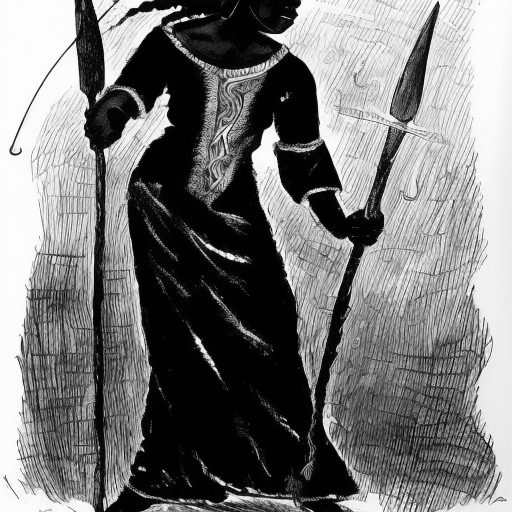
\includegraphics[scale=.6]{advancement/Mystic5}
\end{center}

\begin{multicols*}{2}


\myhighlight{Uncanny}{adv-mystic-uncanny}

Choose one of the following: 1) you take -4 damage from iron weapons (minimum 1); 2) you take -4 damage from wooden weapons (minimum 1); 3) you take -4 damage per die from non-magical fire (minimum 1 per die); 4) you are immune to drowning; 5) you take no damage from falling; 6) you take -4 damage per die from \mylink{Toxins}{malignants-toxins} (minimum 1 per die); 7) you are immune to effects of magical Charm and Sleep.


\cbreak



\myhighlight{Wisdom}{adv-mystic-wisdom}

Advance your \mylink{Juju}{cruces-mojo-juju} \DCUP.

\myhighlight{Witch}{adv-mystic-witch}

Advance your \mylink{Juju}{cruces-mojo-juju} \DCUP. 

\end{multicols*}



\newpage
 %%%%%%%%%%%%%%%%%%%%%%%%%%%%%%%%%%%%%%%%%%%%%%%%%%%%%%%%%%%%%%%%%%%%%%
  %%%%  PHILOSOPHER %%%%%%%%%%%%%%%%%%%%%%%%%%%%%%%%%%%%%%%%%%%%%%%%%%%%%%%
  %%%%%%%%%%%%%%%%%%%%%%%%%%%%%%%%%%%%%%%%%%%%%%%%%%%%%%%%%%%%%%%%%%%%%%

\mysubsection{Philosopher Virtues}{advancement-philosopher-virtues}

\begin{center}
\myredbold{Unless otherwise specified, you can only take each Virtue once.}
\end{center}



  \mytable{Y Y Y} {
    \thead{Daredevil (Level 2+)} & \thead{Heroic (Level 4+)} & \thead{Legendary (Level 7+)} \\
  } {
    Bagman &  Anarchist & Kallisti \\   
    Charms  & Conduit of Blood & Kismet III \\
    Chymist\Asterisk & Doctor & Maestro \\
    Discordian & Esteemed & Patron \\ 
    Kismet I & Kismet II &  Personality III \\
    Medicine & Knowledge is Power & Saves III \\
    Personality I & Personality II &  Staff Magic: Archmage \\
    Professor & Saves II  & Tutor \\
    Sacraments  & Staff Magic: Warlock & - \\
    Saves I  & Well Read & - \\
    Scribe\Asterisk &  - & - \\
    Sorcerer\Asterisk &  - & - \\
    Staff Magic: Novice & - & - \\
}




\callout {
    \Asterisk This Virtue can be taken once per \LVL. See details in description
}


\begin{multicols*}{2}


\myhighlight{Anarchist}{adv-philosopher-anarchist}

You may \mylink{Ride the Tiger}{cruces-blood-ride-the-tiger} in lieu of rolling Blood Dice at any time. Add +2 Blood Dice to the total pool of dice you can channel in this way (i.e. if you have the Virtue: Discordian, you may now channel up to 4 Blood Dice). Once per Session, you may turn a \mylink{Calamity}{table-calamities} you suffer into a \mylink{Mishap}{table-mishap} instead (though the Arcana still fails).

\myhighlight{Bagman}{adv-philosopher-bagman}

Identical to the Virtue of the same name under the \mylink{Philosopher Trope}{trope-philosopher}.

\myhighlight{Charms}{adv-philosopher-charms}

You can perform the \mylink{Charms}{vulgate-charms} Vulgate at will.

\myhighlight{Chymist}{adv-philosopher-chymist}

Identical to the Virtue of the same name under the \mylink{Philosopher Trope}{trope-philosopher}. If you already know this Virtue, gain 1 Research Pip. You may choose this Virtue once per \LVL.

\myimage{advancement/Philosopher4}

\newpage

\myhighlight{Conduit of Blood}{adv-philosopher-conduit-blood}

Once per Session, when rolling your Blood \POOL, you can make every die a natural 6.  Note this might trigger a Mishap, Calamity, or Ruin (see the section on \mylink{Wizardry}{arcana-wizardry}).  If you invoke a Calamity or Ruin when using this Virtue, the spell \mybold{does not fail}, but you still must roll on the appropriate table.

\myhighlight{Discordian}{adv-philosopher-discordian}

   You may \mylink{Ride the Tiger}{cruces-blood-ride-the-tiger} in lieu of rolling Blood Dice at any time. You may channel up to 2 Blood Dice (instead of 1) in this way. Once per Session, you may ignore the effects of any rolls on the \mylink{Mishap Table}{table-mishap}.


\myhighlight{Doctor}{adv-philosopher-doctor}

Advance your \mylink{Ingenuity}{cruces-knowledge} \DCUP. 

\myhighlight{Esteemed}{adv-philosopher-esteemed}

Your wisdom and sound judgment have earned you high respect in "civilized" society. People will often seek you out for your counsel, and enemies consider you a diplomat before they consider you a foe. Even among strangers you are afforded the benefit of the doubt (for example, if you were to be caught up in a mutiny or a crime you might be spared unless you were directly involved). If you are taking \mylink{Downtime}{downtime} in a Medium or Large Settlement, consider the duration of your stay to be one level "cheaper" i.e. treat Months as if they were Weeks, Weeks as Days, and Days as free (staying for Years still incurs the same cost).

\myhighlight{Kallisti}{adv-philosopher-kallisti}

You may \mylink{Ride the Tiger}{cruces-blood-ride-the-tiger} in lieu of rolling Blood Dice at any time. Add +2 Blood Dice to the total pool of dice you can channel in this way (i.e. if you have the Virtue: Discordian and Virtue: Anarchist, you may now channel up to 6 Blood Dice). Once per Session, you may turn a \mylink{Ruin}{table-ruin} you suffer into a \mylink{Calamity}{table-calamities} instead.

\cbreak

\myhighlight{Kismet I-III}{adv-philosopher-kismet}

Advance \mybold{all} aspects of your \mylink{Kismet}{adventurer-kismet} to the next named level (\DEATH, \INJURY, or \INSANITY).

\myhighlight{Knowledge is Power}{adv-philosopher-knowledge-power}

You can cast spells off of Fetishes using your Knowledge Die.

\myhighlight{Maestro}{adv-philosopher-maestro}

Advance your \mylink{Ingenuity}{cruces-knowledge} \DCUP. You may work with the Arbiter to create your own \mylink{Leechcraft}{arcana-leechcraft}.


\myhighlight{Medicine}{adv-philosopher-medicine}

You can perform the \mylink{Medicine}{vulgate-medicine} Vulgate during the \mylink{Shopping Step}{downtime-shopping} of \mylink{Downtime}{downtime}. 

\myhighlight{Patron}{adv-philosopher-patron}

Like Ningauble and Sheelba, young and eager adventurers find their way to your doorstep. During the \mylink{Training Step}{downtime-training} of \mylink{Downtime}{downtime}, an Adventurer seeks you out who is willing to run "errands" for you. They won't work for free and are roughly 1st or 2nd level; depending on how complex the task is, they will return to you in Days, Weeks, or Months (Arbiter's discretion) with whatever you asked for. They won't kill for you, except indirectly (they're not assassins). The Arbiter has final say on whether or not they succeed, but this should be a conversation between the two of you before you send them on their quest. If you betray them (by not paying them, for example) the Arbiter is encouraged to avenge them.

\myhighlight{Personality I-III}{adv-philosopher-personality}

Advance two \mybold{different} aspects of your \mylink{Personality}{adventurer-personality} \DCUP.

\myhighlight{Professor}{adv-philosopher-professor}

Advance your \mylink{Ingenuity}{cruces-knowledge} \DCUP.


\myhighlight{Sacraments}{adv-philosopher-sacraments}

You gain a single Grace die (d4) which allows you to perform the \mylink{Sacraments}{vulgate-sacraments}.

\myhighlight{Saves I-III}{adv-philosopher-saves}

Advance \mybold{all} \mylink{Saves}{adventurer-saves} to the next named level (Defenseless to Preserved; Preserved to Protected; etc).

   \myimage{advancement/ManHat}

\myhighlight{Scribe}{adv-philosopher-scribe}

Identical to the Virtue of the same name under the \mylink{Philosopher Trope}{trope-philosopher}. If you already know this Virtue, gain 1 Research Pip. You may choose this Virtue once per \LVL.

\myhighlight{Sorcerer}{adv-philosopher-sorcerer}

Gain +1 Blood \POOL and choose \mybold{one} of the following:

\mybullet {
    \item One \mylink{Secret}{arcana-wizardry} of your choosing is now inscribed in your skull (see \mylink{Sorcerer's Skull}{arcana-wizardry-skull} for more info). This must be a Secret in your possession (either on a Grimoire or Fetish). 
    \item Automatically scribe three (3) \myital{random} \mylink{Secrets}{arcana-wizardry-secrets} into your Grimoire, provided you have room for them (reminder: a Grimoire can hold up to 10 Secrets). You do not need to know the Virtue of \mylink{Scribe}{trope-philosopher} to write these Arcana. If you roll a Secret already in your Grimoire, roll again (\mylink{Appendix A}{appendix-a} has a random spell table). 
    \item Scribe one \mylink{Secret}{arcana-wizardry-secrets} of your choosing into your Grimoire, provided you have room (reminder: a Grimoire can hold up to 10 Secrets). You do not need to know the Virtue of \mylink{Scribe}{trope-philosopher} to write this Arcana. 
}

You may choose this Virtue once per \LVL.

\myhighlight{Staff Magic: Archmage}{adv-philosopher-staff-archmage}

You may create a \mylink{Staff of the Archmage}{wonder-staff-magic} containing Archmage Powers. Note that this does not grant you the ability to imbue a staff with Novice or Warlock powers.

\myhighlight{Staff Magic: Novice}{adv-philosopher-staff-novice}

Identical to the Virtue of the same name under the \mylink{Philosopher Trope}{trope-philosopher}.

\myhighlight{Staff Magic: Warlock}{adv-philosopher-staff-warlock}

You may create a \mylink{Warlock staff}{wonder-staff-magic} containing Warlock Powers. Note that this does not grant you the ability to imbue a staff with Novice powers.

\myhighlight{Tutor}{adv-philosopher-tutor}

An apprentice joins you.  They are \mylink{Henchmen}{gear-henchmen} with Cowardly morale; they expect nominal pay, room, and board - otherwise, they will need to make periodic Morale checks at the discretion of the Arbiter.  They have 4 Flesh, wear no armor, and can carry up to 8 Burden. Grimoires and Fetishes cost them no Burden to carry, but all other gear they carry counts as double Burden.  In addition, they (a) grant you +3 Research Pips during Downtime; (b) assist you in your Leechcraft so you that only fail Ingenuity tries on 1 instead of 1 or 2; and (c) can take any physical damage for you.  You can only have 1 apprentice at any time.

\myhighlight{Well Read}{adv-philosopher-well-read}

Once per Session, you can declare something to be true because you read it in a book. The base chance of the thing actually being true is 3 in 6. There has to be a plausible way you could know about it from reading books (new discoveries, minor details, and personal secrets are unlikely). You don't know whether or not it is true right away; the Arbiter will roll when it matters. You might only be partially correct, but you will never be catastrophically wrong. If you declare that bugbears fear albino goats, they will either fear albino goats or be indifferent to albino goats. They won't be driven into a murderous rage by them. If you have access to a \mylink{Library}{gear-services} the base chance increases to 5 in 6.

\cbreak

\myimage{advancement/Philosopher5}



\end{multicols*}


\newpage
  %%%%%%%%%%%%%%%%%%%%%%%%%%%%%%%%%%%%%%%%%%%%%%%%%%%%%%%%%%%%%%%%%%%%%%
  %%%%  SELLSWORD %%%%%%%%%%%%%%%%%%%%%%%%%%%%%%%%%%%%%%%%%%%%%%%%%%%%%%%
  %%%%%%%%%%%%%%%%%%%%%%%%%%%%%%%%%%%%%%%%%%%%%%%%%%%%%%%%%%%%%%%%%%%%%%

\mysubsection{Sellsword Virtues}{advancement-sellsword-virtues}

\begin{center}
\myredbold{Unless otherwise specified, you can only take each Virtue once.}
\end{center}


  \mytable{Y Y Y} {
    \thead{Daredevil (Level 2+)} & \thead{Heroic (Level 4+)} & \thead{Legendary (Level 7+)} \\
  } {
    Blademaster & Berserker & Captain \\
    Charms & Boxer & Death Dancer \\
    Deadly & Command & Inspiration \\
    Expertise & Kismet II & Kismet III \\
    Kismet I & Mastery & Mortal Blow \\
    Medicine & Personality II & Personality III \\
    Personality I & Saves II & Righteous Blade \\
    Sacraments  & Sword Saint & Saves III \\
    Saves I  & Survivor & - \\
    Sixth Sense & Valor & - \\
    Three Kills Per Stroke & - & - \\
    Warder & - & - \\
}


\begin{multicols*}{2}

\myhighlight{Berserker}{adv-sellsword-berserker}

If you are \mylink{Dying}{combat-dying}, you may continue to fight.  Gain +4 to Attack and Guard rolls and immunity to the \mylink{Afraid}{effect-afraid} effect.  This bonus instantly ends when you go above 0 Flesh.  While at 0 Flesh, you will still have to roll your \DEATH at the Top of the Moment, and must try your \INSANITY and \INJURY at the end of Combat.

\myhighlight{Blademaster}{adv-sellsword-blademaster}

Identical to the Virtue of the same name under the \mylink{Sellsword Trope}{trope-sellsword}.

\myhighlight{Boxer}{adv-sellsword-boxer}

Your \mylink{Unarmed attacks}{combat-damage-unarmed} do +2 damage. 

\myhighlight{Captain}{adv-sellsword-captain}

4 men-at-arms pledge their blades to your cause. They are \mylink{Mercenaries}{gear-mercenaries} in all ways like \mybold{Meatshields}, except they have a starting Loyalty of 9 and wear Light Armor. They can each carry up to 6 \mylink{Burden}{gear-burden} of gear. The require no pay or compensation, other than food (including providing Provisions during a \mylink{Bivouac}{combat-resting-bivouac}). They will not tolerate other \mylink{Mercenaries}{gear-mercenaries} in your Band, unless they have been hired by another Adventurer. You have to specify what each man-at-arms is doing at the top of each Moment i.e. "2 are giving me +1 to Fight, 1 is giving me +1 damage, and I'm keeping one back to take damage in case things go south."  If a man-at-arms dies or leaves your service, they will be replaced with another during the \mylink{Production Step}{downtime-production} of \mylink{Downtime}{downtime}. Note that if your men-at-arms often meet with an untimely end, starve to death, leave your service, etc. you may begin to develop a ... reputation ... at the Arbiter's discretion.


\myhighlight{Charms}{adv-sellsword-charms}

You can perform the \mylink{Charms}{vulgate-charms} Vulgate at will.

\myhighlight{Command}{adv-sellsword-command}

Make an \RSTRY{\PRE} at the top of the Moment. If you succeed, you can immediately rally your Allies as a Combat Action (meaning the Rallying Cry ends your turn).  All Allies win Init and gain +4 to Attack and Guard rolls until the bottom of the Moment. You can do this as many times in Combat as you like, but you must \RSTRY{\PRE} each time. 

\myhighlight{Deadly}{adv-sellsword-deadly}

Identical to the Virtue of the same name under the \mylink{Sellsword Trope}{trope-sellsword}.

\myhighlight{Death Dancer}{adv-sellsword-death-dancer}

Gain +6 \MAX Grit.  Once per Session, you can use a Combat Action to kill every Monster in Close range provided they have 2 \HD or less.  If you do a good job describing this to the Arbiter, it will prompt a Morale check in any Nearby Monsters if they have 4 \HD or less.  

\myhighlight{Expertise}{adv-sellsword-expertise}

Advance your \mylink{Prowess}{sellsword-prowess} \DCUP.

\myhighlight{Inspiration}{adv-sellsword-inspiration}

Advance your \mylink{Prowess}{sellsword-prowess} \DCUP.


\myhighlight{Kismet I-III}{adv-sellsword-kismet}

Advance \mybold{all} aspects of your \mylink{Kismet}{adventurer-kismet} to the next named level (\DEATH, \INJURY, or \INSANITY).

\myhighlight{Mastery}{adv-sellsword-mastery}

Advance your \mylink{Prowess}{sellsword-prowess} \DCUP.

\myhighlight{Medicine}{adv-sellsword-medicine}

You can perform the \mylink{Medicine}{vulgate-medicine} Vulgate during the \mylink{Shopping Step}{downtime-shopping} of \mylink{Downtime}{downtime}. 

\myhighlight{Mortal Blow}{adv-sellsword-mortal-blow}

Once only, you may sacrifice your life to either save the life of another, or deal a killing blow to a Monster. If you are saving someone's life, they must be Close to you; if you are dealing a killing blow, you must be able to affect the Monster (Magic to hit, etc.). The amount of Health the Monster possesses has no bearing on the killing blow. Upon your demise, your soul travels to \mylink{Limbo}{the-afterlife} as normal. No Virtue short of \mylink{Norn's Shears}{adv-mystic-norns-shears} can save your life, but you will remain "barely alive" until the end of Combat, giving you a chance to say some epic last words.  Make 'em count.

\myhighlight{Personality I-III}{adv-sellsword-personality}

Advance two \mybold{different} aspects of your \mylink{Personality}{adventurer-personality} \DCUP.

\myhighlight{Righteous Blade}{adv-sellsword-righteous-blade}

Any weapon you use (including if you are fighting Unarmed) is considered Magical.

\myhighlight{Sacraments}{adv-sellsword-sacraments}

You gain a single Grace die (d4) which allows you to perform the \mylink{Sacraments}{vulgate-sacraments}.

\myhighlight{Saves I-III}{adv-sellsword-saves}

Advance \mybold{all} \mylink{Saves}{adventurer-saves} to the next named level (Defenseless to Preserved; Preserved to Protected; etc).

\myhighlight{Sixth Sense}{adv-sellsword-sixth-sense}

Gain +6 \MAX Grit. No one can get \mylink{the Drop}{combat-drop} on you.  

\myhighlight{Survivor}{adv-sellsword-survivor}

Once per Session, if you're in a wilderness setting, you can say that you know of a cache nearby hidden in a tree bole, under a cairn, etc.  The cache can contains one of: 1) \UDD{d8} of food and water; 2) a \mylink{Bow}{gear-dex-weapons} with \UDD{d8} of arrows; 3) a suit of normal sized Light Armor; 4) a war axe, spear, and set of 4 daggers; 5) a small minor item (lantern and a few flasks of oil, OK; vials of poison or a looking glass, not OK).

\myhighlight{Sword Saint}{adv-sellsword-sword-saint}

Any \VIG weapon you wield deals \DCUP damage.

\myhighlight{Valor}{adv-sellsword-valor}

Gain +6 \MAX Grit. You are immune to being \mylink{Afraid}{effect-afraid}.  


\myhighlight{Three Kills per Stroke}{adv-sellsword-three-kills}

Identical to the Virtue of the same name under the \mylink{Sellsword Trope}{trope-sellsword}.


\cbreak

\myimage{advancement/Sellsword3}

\myhighlight{Warder}{adv-sellsword-warder}

Choose an Ally at the start of Combat.  You must keep that Ally Close to you. If that ally would take damage from a physical attack, you can choose to take the damage for them instead.

\end{multicols*}




\newpage
\mysection{Species}{advancement-species}
  %%%%%%%%%%%%%%%%%%%%%%%%%%%%%%%%%%%%%%%%%%%%%%%%%%%%%%%%%%%%%%%%%%%%%%
  %%%%  MURK %%%%%%%%%%%%%%%%%%%%%%%%%%%%%%%%%%%%%%%%%%%%%%%%%%%%%%%
  %%%%%%%%%%%%%%%%%%%%%%%%%%%%%%%%%%%%%%%%%%%%%%%%%%%%%%%%%%%%%%%%%%%%%%

\mysubsection{Murk Virtues}{advancement-murk-virtues}

\begin{center}
\myredbold{Unless otherwise specified, you can only take each Virtue once.}
\end{center}

  \mytable{Y Y Y} {
    \thead{Daredevil (Level 2+)} & \thead{Heroic (Level 4+)} & \thead{Legendary (Level 7+)} \\
  } {
    Apprentice of the Bride & Footpad of the Bride & Kismet III \\
    Ghost & Invisibility & Loner \\
    Kismet I &  Kismet II &  Personality III \\
    Mortal Charms & Personality II  &  Saves III \\
    Personality I & Saves II & Sharper of the Bride \\
    Saves I & Self-Reliant & Stonewalker\\
    Self-Sufficient & Shadowblade & -  \\
    Stonespeaker & Stoneshaper & - \\
    Will to Live  & - & - \\
    You and Me  & -  & - \\
}



\begin{multicols*}{2}

\myhighlight{Apprentice of the Bride}{adv-murk-bride}

Advance \mylink{Whispers of the Bride}{vulgate-whisper-the-bride} from Untrained to Apprentice (d4) rank.

\myhighlight{Footpad of the Bride}{adv-murk-footpad}

Advance \mylink{Whispers of the Bride}{vulgate-whisper-the-bride} from Apprentice to Footpad (d6) rank.


\myhighlight{Ghost}{adv-murk-ghost}

Mortals tend to forget you're there. They can never seem to remember your face (though they'll remember "a shadowy figure" of some sort); they don't speak to you unless you speak first, you tend to startle them when you come up to them. This means that \mybold{if (and only if) a Mortal is alone}, you can come right up to them and put a hand on their shoulder (or a knife in their back) without them noticing you're there (meaning you would get \mylink{the Drop}{combat-drop} on them). 

\myhighlight{Invisibility}{adv-murk-invisibility}

Once per Session, you can step into a shadow and become \mylink{Invisible}{effect-invisible}.  You can use this to get \mylink{the Drop}{combat-drop} on someone, but there must be a shadow present (you couldn't do this in the middle of a sunny field, for example).

\myhighlight{Kismet I-III}{adv-murk-kismet}

Advance \mybold{all} aspects of your \mylink{Kismet}{adventurer-kismet} to the next named level (\DEATH, \INJURY, or \INSANITY).

\myhighlight{Loner}{adv-murk-loner}

Gain +4 \MAX Grit. Once per Session, if you are completely by yourself, you can treat a \mylink{Breather}{combat-resting-breather} as if you had taken a \mylink{Bivouac}{combat-resting-bivouac}. You must make your Provisions roll if applicable. 

\myhighlight{Mortal Charms}{adv-murk-mortal-charms}

You can perform the \mylink{Charms}{vulgate-charms} Vulgate at will.

\myhighlight{Personality I-III}{adv-murk-personality}

Advance two \mybold{different} aspects of your \mylink{Personality}{adventurer-personality} \DCUP.

\myhighlight{Saves I-III}{adv-murk-saves}

Advance \mybold{all} \mylink{Saves}{adventurer-saves} to the next named level (Defenseless to Preserved; Preserved to Protected; etc).

\myhighlight{Self-Reliant}{adv-murk-self-reliant}

Gain +4 \MAX Grit. Restore an additional +4 Grit when you take a \mylink{Breather}{combat-resting-breather} up to your \MAX, unless a \mylink{Injury}{adventurer-kismet-injury} prevents you from doing so).


\myhighlight{Self-Sufficient}{adv-murk-self-sufficient}

Gain +4 \MAX Grit. You never need to roll \mylink{Provisions}{gear-equipment} when taking a \mylink{Bivouac}{combat-resting-bivouac}.

\myhighlight{Shadowblade}{adv-murk-shadowblade}

You can reach into a shadow and pull out a long, ebony dagger that appears to be made of black vapor. The weapon exists for as long as it is not exposed to sunlight.  The dagger is magical and does d10 damage, and can have Toxins applied to it.  If the dagger takes a life it immediately disappears into the Void, bearing the soul of the slain creature with it forever.

\myhighlight{Sharper of the Bride}{adv-murk-sharper}

Advance \mylink{Whispers of the Bride}{vulgate-whisper-the-bride} from Footpad to Sharper (d8) rank.

\cbreak

\myhighlight{Stoneshaper}{adv-murk-stone-shaper}

Once per Session, you can speak to stones and have them reshape themselves.  The stones can't be bigger than 3m in any dimension.  The stone will reshape itself into anything you desire - a large rock could be shaped into an idol, a passage could be made through a wall (provided the wall was less than 3m thick).  The object created is rough-hewn - fine detail isn't possible (Arbiter's discretion)


\myhighlight{Stonespeaker}{adv-murk-stone-speaker}

In addition to the \mylink{Silent Speech}{idiolect-silent-speech}, you can convince the stones to move by speaking with them for Minutes. They can't do anything rocks wouldn't be able to do (float on water, fly through the air without being thrown, etc.), but you can convince them to roll, "walk", fall, or move out of the way.

\myhighlight{Stonewalker}{adv-murk-stonewalker}

Once per Session, you can travel through stone or earth up 10km away. You need to have visited the destination and there must be uninterrupted stone or ground between yourself and the destination. You can travel this distance in Minutes. When you reach level 9, you can use this ability to return to \mylink{Svartalfheim}{species-murk} if you choose (retiring your character).

\myhighlight{Will to Live}{adv-murk-will-to-live}

You only fail your \DEATH try on a 1 (instead of a 1 or 2).

\myhighlight{You and Me}{adv-murk-you-and-me}

When fighting a single combatant, you gain +4 damage and a +4 bonus to any \mylink{Combat Actions}{combat-combat-actions} provided there is no one else Close to you (Ally or Monster). This bonus immediately ends if any additional Ally or Monster comes Close to you, and won't return for the rest of Combat.

\end{multicols*}

\newpage
%%%%%%%%%%%%%%%%%%%%%%%%%%%%%%%%%%%%%%%%%%%%%%%%%%%%%%%%%%%%%%%%%%%%%%
%%%%  NIGHT CHILDREN %%%%%%%%%%%%%%%%%%%%%%%%%%%%%%%%%%%%%%%%%%%%%%%%%%%%%%%
%%%%%%%%%%%%%%%%%%%%%%%%%%%%%%%%%%%%%%%%%%%%%%%%%%%%%%%%%%%%%%%%%%%%%%
\mysubsection{Night Child Virtues}{advancement-night-child-virtues}

\myemph{Unless otherwise specified, you can take each Virtue only once.}


  \mytable{Y Y Y} {
    \thead{Daredevil (Level 2+)} & \thead{Heroic (Level 4+)} & \thead{Legendary (Level 7+)} \\
  } {
    Freaky\Asterisk  & Bump\Asterisk  & Kismet III \\
    Kismet I & Bump Bump\Asterisk  &  Nuke\\
    More Freaky\Asterisk  &  Bump Bump Bump\Asterisk  &  Personality III \\
    More Pretty\Asterisk  & Bump Bump Bump Bump\Asterisk   &  Saves III \\
    More Stuff\Asterisk  & Kismet II & That One\Asterisk  \\
    Personality I & Personality II & - \\
    Pretty\Asterisk  & Saves II & -  \\
    Saves I & - & - \\
    Stuff\Asterisk   & - & - \\
}

\callout {
    \Asterisk This Virtue can be taken up to three times per \LVL.
}


\begin{multicols*}{2}

\myhighlight{Bump}{adv-night-child-bump}

Add or subtract 1 to a Looks, Weird, or Gear roll you just made.

\myhighlight{Bump Bump}{adv-night-child-bump-bump}

Add or subtract 2 to a Looks, Weird, or Gear roll you just made.

\myhighlight{Bump Bump Bump}{adv-night-child-bump-bump-bump}

Add or subtract 3 to a Looks, Weird, or Gear roll you just made.

\myhighlight{Bump Bump Bump Bump}{adv-night-child-bump-bump-bump-bump}

Add or subtract 4 to a Looks, Weird, or Gear roll you just made.


\myhighlight{Freaky}{adv-night-child-freaky}

Roll your Weird die and apply the result to your Adventurer.

\cbreak

\myhighlight{Kismet I-III}{adv-night-child-kismet}

Advance \mybold{all} aspects of your \mybold{Kismet} - \DEATH, \INJURY, and \INSANITY - to the next named level.


\myhighlight{More Freaky}{adv-night-child-more-freaky}

Raise you Weird die \DCUP.

\myhighlight{More Pretty}{adv-night-child-more-pretty}

Raise you Looks die \DCUP.

\myhighlight{More Stuff}{adv-night-child-more-stuff}

Raise you Gear die \DCUP.

\end{multicols*}
\newpage

\begin{center}
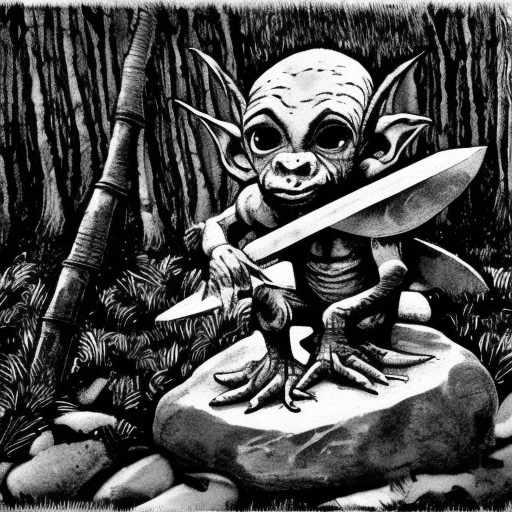
\includegraphics{advancement/NightChild}
\end{center}

\begin{multicols*}{2}

\myhighlight{Nuke}{adv-night-child-nuke}

At any time, you may open yourself to the Void, channeling it through your body. Roll your Looks, Weird, and Gear dice and deal \SUM x2 damage to all Monsters Close or Nearby (Save for half damage). After you roll the damage, immediately roll on the \mypg{Ruin}{table-ruin} table.

\myhighlight{Personality I-III}{adv-night-child-personality}

Advance two \mybold{different} aspects of your \mybold{Personality} \DCUP. 


\myhighlight{Pretty}{adv-night-child-pretty}

Roll your Looks die and apply the result to your Adventurer.

\cbreak

\myhighlight{Saves I-III}{adv-night-child-saves}

Advance \mybold{all} Saves to the next named level (Defenseless to Preserved; Preserved to Protected; etc). 

\myhighlight{Stuff}{adv-night-child-stuff}

Roll your Gear die and apply the result to your Adventurer.

\myhighlight{That One}{adv-night-child-that-one}

Choose a Looks, Weird, or Gear result as if you rolled the appropriate die.  For example, if your Gear die is a d8, you can choose any Gear result from 1 to 8.

\end{multicols*}

\newpage
%%%%%%%%%%%%%%%%%%%%%%%%%%%%%%%%%%%%%%%%%%%%%%%%%%%%%%%%%%%%%%%%%%%%%%
%%%%  POOKA %%%%%%%%%%%%%%%%%%%%%%%%%%%%%%%%%%%%%%%%%%%%%%%%%%%%%%%
%%%%%%%%%%%%%%%%%%%%%%%%%%%%%%%%%%%%%%%%%%%%%%%%%%%%%%%%%%%%%%%%%%%%%%

\mysubsection{Pooka Virtues}{advancement-pooka-virtues}

\begin{center}
\myredbold{Unless otherwise specified, you can only take each Virtue once.}
\end{center}


  \mytable{Y Y Y} {
    \thead{Daredevil (Level 2+)} & \thead{Heroic (Level 4+)} & \thead{Legendary (Level 7+)} \\
  } {
    Apprentice of the Rabbit & Epic Songs & Icon \\
    Calling in the Markers & Fast Metabolism &  Kismet III \\
    Healing Wax &  Footpad of the Rabbit &  Martyrdom \\
    Kismet I & Kismet II  &  Personality III \\
    Laugh it Off & Personality II & Saga of Heroes \\
    Mascot & Rager & Saves III \\
    Must Be My Lucky Day! & Saves II & Sharper of the Rabbit  \\
    Personality I & Talisman & - \\
    Saves I  & Wound Transfer & - \\
    Two Murks Walk Into a Bar... & - & - \\
}


\begin{multicols*}{2}


\myhighlight{Apprentice of the Rabbit}{adv-pooka-apprentice-rabbit}

Advance \mylink{Whispers of Br'er Rabbit}{vulgate-whisper-brer-rabbit} from Untrained to Apprentice (d4) rank.

\myhighlight{Calling in the Markers}{adv-pooka-markers}

During the \mylink{Shopping Step}{downtime-shopping} of \mylink{Downtime}{downtime}, you can roll your \LUCK. You gain up to \SUM items from the \mylink{Tools}{gear-equipment} list, as long as the total cost doesn't exceed \SUM x10 gold.  If you wish, you can distribute this gear immediately to the rest of your Band.

\myhighlight{Epic Songs}{adv-pooka-epic-songs}

When using your \mylink{Hype Man}{pooka-virtue-hype-man} Virtue, you roll a d8 for each member of your Band (including yourself).

\myhighlight{Fast Metabolism}{adv-pooka-fast-metabolism}

You are immune to \mylink{Toxins}{malignants-toxins}, \mylink{Curses}{cunning-curses}, and \mylink{Diseases}{vulgate-medicine-diseases} of all sorts.

\begin{center}
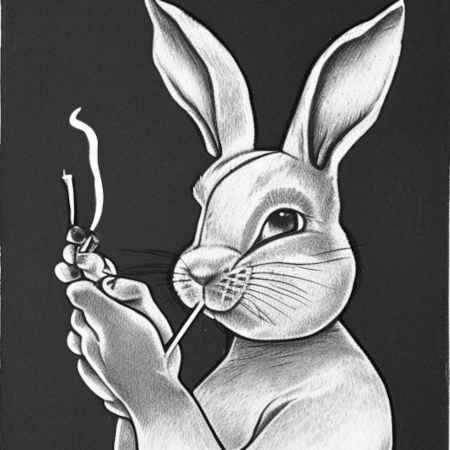
\includegraphics[scale=.4]{advancement/Pooka2}
\end{center}

\newpage

\myhighlight{Footpad of the Rabbit}{adv-pooka-footpad-rabbit}

Advance \mylink{Whispers of Br'er Rabbit}{vulgate-whisper-brer-rabbit} from Apprentice to Footpad (d6) rank.


\myhighlight{Healing Wax}{adv-pooka-healing}

Once per Session, you can pull a glob of wax out of your ear.  Anyone who eats it restores 4 Flesh (up to \MAX). If no one consumes it by the end of the Session, it just becomes a "normal" lump of ear wax.

\myhighlight{Icon}{adv-pooka-icon}

Advance your \mylink{Lucky Die}{pooka-lucky-die} \DCUP.

\myhighlight{Kismet I-III}{adv-pooka-kismet}

Advance \mybold{all} aspects of your \mylink{Kismet}{adventurer-kismet} to the next named level (\DEATH, \INJURY, or \INSANITY).

\myhighlight{Laugh it Off}{adv-pooka-laugh-it-off}

Once per Session, you may make it so that any physical blow that would hit you misses instead.  This has to be plausible and luck based: "I slipped and fell just as the sword came down and it missed me", for instance.  You can choose to "laugh it off" after the damage is rolled.

\myhighlight{Martyrdom}{adv-pooka-martyrdom}

If a Mortal Ally dies, you can take their place.  The Ally needs to be Close or Nearby to you, and they cannot have been dead for longer than Hours.  The body of the Mortal must be in reasonably good shape - you can't save them if they've been reduced to ashes, for example.  You immediately disappear into the Void and the Ally's soul returns immediately to its body. Those who have been saved by Pooka are said to take on some of their "personality".

\myhighlight{Mascot}{adv-pooka-mascot}

Advance your \mylink{Lucky Die}{pooka-lucky-die} \DCUP.

\myhighlight{Must Be My Lucky Day!}{adv-pooka-lucky-day}

 Once per \mylink{Session}{time-session}, you can do 1 of the following:  (a) win any game of chance; (b) find extra Narcotics just lying around (d2 \UD of any Narcotic you want - if you don't use it before the next Session, it gets lost or evaporates or whatever); (c) find a \mylink{Tool}{gear-equipment} you might need lying on the ground. The tool can only be used once before it breaks, is used up, etc.; or (d) regain 1 Flesh (enough to bring you off Death's Door).

\myimage{advancement/LittleWitch}


\myhighlight{Personality I-III}{advancement-pooka-personality}

Advance two \mybold{different} aspects of your \mylink{Personality}{adventurer-personality} \DCUP.

\myhighlight{Rager}{adv-pooka-rager}

Once per Session, you can host a Rager during a \mylink{Bivouac}{combat-resting}.  Every person who participates will gain the effects of the \mylink{Resting Step}{downtime-resting} of \mylink{Downtime}{downtime}. The following morning, everyone must make an \RSTRY{\VIG}. If they fail they are \mylink{Hung Over}{effect-hung-over}.

\newpage

\myhighlight{Saga of Heroes}{adv-pooka-saga-heroes}

When using your \mylink{Hype Man}{pooka-virtue-hype-man} Virtue, you roll a d10 for each member of your Band (including yourself).

\myhighlight{Saves I-III}{adv-pooka-saves}

Advance \mybold{all} \mylink{Saves}{adventurer-saves} to the next named level (Defenseless to Preserved; Preserved to Protected; etc).

\myhighlight{Sharper of the Rabbit}{adv-pooka-sharper-rabbit}

Advance \mylink{Whispers of Br'er Rabbit}{vulgate-whisper-brer-rabbit} from Footpad to Sharper (d8) rank.

\myhighlight{Talisman}{adv-pooka-talisman}

Advance your \mylink{Lucky Die}{pooka-lucky-die} \DCUP.

\myhighlight{Two Murks Walk Into a Bar...}{adv-pooka-two-murks}

When using your \mylink{Hype Man}{pooka-virtue-hype-man} Virtue, you roll a d6 for each member of your Band (including yourself).

\myhighlight{Wound Transfer}{adv-pooka-wound-transfer}

You can transfer your Flesh to Allies on a 1-to-1 basis i.e. for every point of Flesh you transfer, you take 1 point of Flesh damage. You do not need to be touching the Ally, but you do need to be Close to them.  The wounds that appear on your body match the wounds taken by the Ally.  The point of Flesh transferred is enough to keep an Ally from Dying.

\end{multicols*}

\newpage
 \mysection{The Spriggan}{species-spriggan}

   \flavor{"Is it not enough?" he said in his strange rich magical voice, and pointed across his wide lands with the fingers that summoned wonder. ~\\ ~\\ She sighed: it was not enough. \Tilde Lord Dunsany} 

\begin{center}
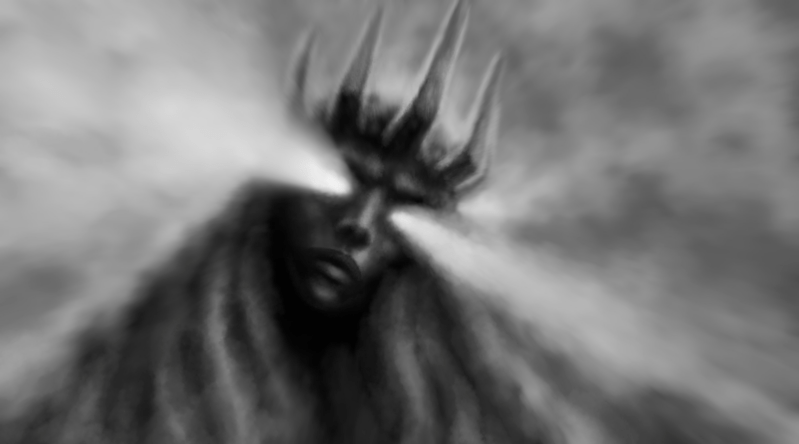
\includegraphics[width=\linewidth,keepaspectratio=true]{species/Spriggan1}
\end{center}

\begin{multicols*}{2}\raggedcolumns

  \mysubsection{Appearance}{spriggan-appearance}
  
  You hail from Elfland, beyond the reach of death.  Like your brothers and sisters the \Murk you are the Nomadic People, the Rom - cursed with curiosity and infected with the fire that burns in the hearts of the Hallowed to know more, to see the passage of time, and to breathe the air of decay.  All it cost was your soul.  

  You cannot find your way home again, for the bright line between this world and Elfland ebbs forever before you.  Wherever you are is where Elfland cannot be.

  Your bloodline allows you to strike bargains with the lowest of the Small Gods, the Forgotten who stand at the threshold of the void.  The fear of oblivion dominates every desire and scheme of these sanguinary spirits.  You steal them away from the doorway of nothingness and by Remembering them, allow them to touch reality once again.  In Remembering, you allow their souls to mingle inside of you, and sing through you - so that in the never-ending ache of the Mortal realm you might, for a moment, remember the feel of the heat of Elfin hearths and the smell of the lavender fields you dream of.  

  You are tall, lithe, and ethereal; Spriggan often stand over 2m, with leaf-shaped ears, long fingers, and gaunt faces vaguely reminiscent of deer or goats.  Older Spriggan often appear cadaverous - while you can't die from old age, your body begins to rot outside of the realm of Elfland (this has no effect on your powers).  Your skin and eye color is as varied as the Mortal races, and from a distance you might pass for human - except for the horns.  Some are small, barely noticeable stubs while other Spriggan sprout deer antlers, curling ram's horns, or tree branches.  It is not uncommon for birds to roost on your horns if they are well developed enough.


  \mysubsection{Creation}{spriggan-creation}

  \callout {
    \mynumlist {
        \item You start with \mybold{6 Flesh and 4 Grit}.
        \item Move your \AWA \DCUP (to a d6).
        \item If you need to \RS:\AWA, you only fail on a natural 1 (instead of a 1 or 2). Put a check next to \AWA on your \mylink{Adventurer Sheet}{adventurer-sheet.10} so you don't forget.
        \item Write down your \mylink{Virtues}{spriggan-virtues}.
        \item Write down your \mylink{Complication}{spriggan-complications}.
        \item Write down your \mylink{Starting Gear}{spriggan-starting-gear}.
    }
 }



  \mysubsection{Spriggan Virtues}{spriggan-virtues}

 \myhighlight{Sovereignty}{spriggan-virtues-sovereignty}

  Though you have been cast out of Elfland, the noble blood of the King of Elfland still runs through your veins.  You may use this sanguine supremacy to summon and command \mylink{the Abandoned}{forgotten-abandoned} and \mylink{the Obliterated}{forgotten-obliterated} (collectively known as  \mylink{the Forgotten}{the-forgotten}), ghosts who live at the edge of oblivion.

The Abandoned are Small Gods whose names have disappeared from the tongues of men; they exist only as a line in a book buried by the sands of the deserts, etched on forgotten stela in the wilderness, or inscribed on scrimshaw lost beneath the waves.  When an Abandoned's name is finally lost, they become the Obliterated - totems and symbols of what they once were, raw power in the form of beasts (through the \mylink{Fealty of the Beasts}{forgotten-fealty-beasts}), elementals (through the \mylink{Fealty of the Elements}{forgotten-fealty-elements}), and devils (through the \mylink{Fealty of the Damned}{forgotten-fealty-damned}).


Your power over the Forgotten is manifest in your Sovereignty.  

\callout{You begin with a Sovereignty of 1, and your \MAX Sovereignty is 9.}
  

  \myhighlight{Remembrance of Elfland}{spriggan-virtues-remembrance-elfland}

  One of the names of the Abandoned exists in your memory. If you know which Abandoned you want to serve you when you first begin, you can name them immediately - otherwise, you can name them at any point in the campaign (when they hopefully appear in your time of need!). Once you name your Abandoned, you cannot change - it is as if you had always known its name, and suddenly remembered it. See the section on \mylink{The Abandoned}{forgotten-abandoned} for more info.

    
  \myhighlight{Fealty of the Beasts}{spriggan-virtues-fealty-beasts}

   You know the ways of summoning and commanding Sprites and more powerful zoological monsters. See the section \mylink{Fealty of the Beasts}{forgotten-fealty-beasts} under \mylink{The Forgotten}{the-forgotten}.

\myhighlight{Sword Magic}{spriggan-virtues-sword-magic}

  You know the wondrous ways of enchanting blades through \mylink{Sword Magic}{wonder-sword-magic}. 

  \myhighlight{Tongues}{spriggan-virtues-tongues}

  You know how to speak all \mylink{Idiolects and Dialects}{civilization-languages}.


  \myhighlight{Undreamt}{spriggan-virtue-undreamt}

  You stand outside of the Dream and are thus untouched by Sish, the Handmaiden of Time. You are immune to aging of any kind, and your \DEATH starts at Tough (d4).

\newpage

  \mysubsection{Complications}{spriggan-complications}

  \myhighlight{Alien}{spriggan-complication-alien}

  As far as Mortals are concerned, you are deeply and fundamentally \myital{weird}. You are eerie and alien, and it's not uncommon for other creatures to react to your presence with fear or loathing. Dogs bark at your approach, a cold breeze seems to follow you, you don't blink enough and your smile never seems to touch your eyes. You are one of the Rom, the Nomadic People - and there are no campfires where you will find welcome, save with your Band.

  \myhighlight{Antlers}{spriggan-complication-antlers}

  Antlers or tree branches grow from your head; birds often roost there (and if they do, you can speak with them). You can't wear helmets or use a \mylink{Bow}{gear-weapons} or \mylink{Strongbow}{gear-weapons}. You can't attack with your antlers, but you can sacrifice them for the same effect as wearing a \mylink{Helmet}{gear-armor}. Antlers will regrow during \mylink{Downtime}{downtime}.

  \myhighlight{Iron allergy}{spriggan-complication-iron-allergy}
    
    Prolonged bare-skin exposure to iron causes severe burns and painful blisters. Touching iron with your bare skin feels like picking up something uncomfortably hot; holding something made of iron for longer than a few Moments is impossible. If you are holding something made of iron with your bare hands, take 1 point of Flesh damage at the top of the next (and every following) Moment. 

  \myhighlight{Unseelie}{spriggan-complication-unseelie}
    
  You are creature of Chaos, one of the \mylink{Unseelie}{the-inhabitants} - and are thus \mybold{Unhallowed}.


  \mysubsection{Starting Gear}{spriggan-starting-gear}

  \callout{\footnotesize{
  You begin with:

  \mybullet {
    \item a pair of leather workgloves;
    \item two silver \mylink{Daggers}{gear-dex-weapons} OR a \mylink{Spear}{gear-vig-weapons}; 
    \item \UDD{d4} of \mylink{Personal Provisions}{gear-equipment};
    \item a set of prayer candles;
    \item a block of salt (for licking) and a pouch of dead mice;
    \item a pouch of 3 gems (roll on the \mylink{Gems table}{appendix-a-gems} in Appendix A)
    \item one pick OR 3 rolls on the \mylink{Random Items}{appendix-a-random-items} table in Appendix A;
  }
}}

    \myhighlight{What Next?}{spriggan-what-next}

    To better understand how you wield \mylink{the Forgotten}{the-forgotten}, read the chapter on \mylink{Remembrance}{remembrance}. You should also take a peek at how to make magical weapons through the Wonder of \mylink{Sword Magic}{wonder-sword-magic}.

\myimage{species/Spriggan2}

\end{multicols*}


\newpage

\begin{multicols*}{2}


}%
